% !TEX root = sum1.tex
\section{Introduction}

\subsection{Background}
Governments worldwide have been faced with the challenge of reducing the spread of Covid-19 while minimizing the economic impact. Social distancing has been widely implemented as the most effective non-pharmaceutical treatment to reduce the health effects of the virus. This website records a timeline of Covid-19 and the relevant epidemic prevention measures \cite{Covid19Timeline}. 

For instance, in March 2020, the Hong Kong government implemented restrictive measures such as banning indoor and outdoor gatherings of more than four people, requiring restaurants to operate at half capacity. As the epidemic worsened, the government tightened measures by limiting public gatherings to two people per group in July 2020. As the epidemic subsided, the Hong Kong government gradually relaxed social distancing restrictions, allowing public group gatherings of up to four people in September 2020. In October 2020, pubs were allowed to serve up to four people per table, and restaurants could serve up to six people per table. Specifically, the Hong Kong government also implemented different measures in different venues \cite{Gov202209}.

For example, the catering businesses will have different social distancing requirements depending on their mode of operation for dine-in services. They can operate at 50\%, 75\%, or 100\% of their normal seating capacity at any one time, with a maximum of 2, 2, or 4 people per table, respectively. Bars and pubs may open with a maximum of 6 persons per table and a total number of patrons capped at 75\% of their capacity. The restrictions on the number of persons allowed in premises such as cinemas, performance venues, museums, event premises, and religious premises will remain at 85\% of their capacity.

The measures announced by the Hong Kong government mainly focus on limiting the number of people in each group and the seat occupancy rate. However, implementing these policies in operations can be challenging, especially for venues with fixed seating layouts. In our study, we will focus on addressing this challenge in commercial premises, such as cinemas and music concert venues. We aim to provide a practical tool for venues to optimize seat assignments while ensuring the safety of groups by proposing a seat assignment policy that takes into account social distancing requirements and the given seating layout. We strive to enable venues to implement social distancing measures effectively by offering a solution that provides specific seating arrangements.


\subsection{Seat Planning and Seat Assignment}
According to the social distancing requirement imposed by the government, the size of the largest group is confined, people in the same group can sit together and the adjcent groups should keep distance with each other.

Then, we clarify the terms, seat planning and seat assignment which will be used in the following parts. In our context, the seat planning means the seat partition in the planning. It includes two forms, fixed seat planning and flexible seat planning. The former one is that some seats are unavailable, they may be dismantled or disabled by staff beforehand. The latter one represents the current seat planning, but the planning can be altered later when the planned seats don't match with the size of a coming group or when the seat planning is disrupted after assigning a coming group. In the seat assignment, for the coming group, when accepting it, we assign the seats to the group, and the seats will not be used by others in the future.

The following picture illustrates the difference.

\begin{figure}[htbp]
    \centering
    \begin{minipage}[t]{0.48\textwidth}
    \centering
    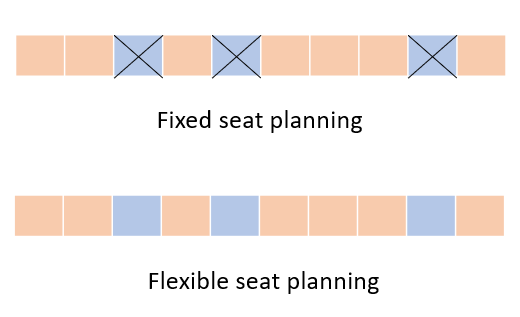
\includegraphics[width=5cm]{./Figures/seat_planning.png}
    \caption{Seat Planning}
    \end{minipage}
    \begin{minipage}[t]{0.48\textwidth}
    \centering
    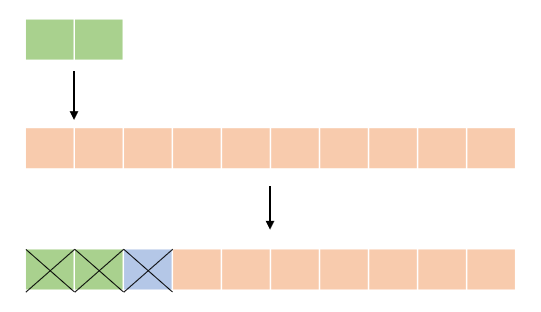
\includegraphics[width=5cm]{./Figures/seat_assignment.png}
    \caption{Seat Assignment}
    \end{minipage}
\end{figure}

We consider to obtain the seat planning with deterministic and stochatic demand. For the deterministic situation, we have complete and accurate information about the demand for seating. We aim to provide a seat planning that maximizes the number of people accommodated. This situation is applicable in venues like churches or company meetings, where fixed seat layouts are available, and the goal is to assign seats to accommodate as many people as possible within the given layout.

% This situation corresponds to the basic problem of assigning more people with the fixed seat layout, such as in a church, a company meeting. It applies in the place where the seat has been provided in advance in case people don;t follow the rules.

For the stochastic situation, we have knowledge of the demand distribution before the actual demand is realized. We aim to generate a seat planning that maximizes the expected number of people accommodated. This approach is suitable for venues where seats have been pre-allocated to ensure compliance with social distancing rules. By considering the expected demand distribution, we can optimize the seat planning to accommodate the maximum number of people while maintaining social distancing.

Regarding the seat assignment, we consider the dynamic demand under the fixed and flexible seat planning. For the dynamic situation, the decision to accept or reject a group is made for each incoming group based on specific requirements. According to the different requirements, we can assign the seats in two forms. Under the fixed seat planning, the fixed seats will be disabled beforehand in case someone don't obey the social distancing rule. Under the flexible seat planning, we can allocate seats immediately upon arrival or at a later time. This situation is commonly encountered in venues such as cinemas or music concerts, where decisions can be made on a group-by-group basis. The goal is to make timely decisions regarding seat assignments, considering factors such as available seating capacity, social distancing requirements and the specific size of each group.


\subsection{Seat Planning with Social Distancing}
We incorporate the social distancing in the seat planning problem. Consider a seat layout comprising $N$ rows, with each row containing $L_j^0$ seats, where $j \in \mathcal{N} \coloneqq \{1,2, \ldots, N\}$. The seating arrangement is used to accommodate various groups, where each group consists of no more than $M$ individuals. There are $M$ distinct group types, denoted by group type $i$, where each group type consists of $i$ people. The set of all group types is denoted by $\mathcal{M} \coloneqq \{1, 2, \ldots, M\}$. The demand for each group type is represented by a demand vector $\mathbf{d} = (d_1, d_2, \ldots, d_M)^{\intercal}$, where $d_i$ represents the number of group type $i$.


In order to comply with the social distancing requirements, individuals from the same group must sit together, while maintaining a distance from other groups. Let $\delta$ denote the social distancing, which could entail leaving one or more empty seats. Specifically, each group must ensure the empty seat(s) with the adjacent group(s).

To model the social distancing requirements into the seat planning process, we add the parameter, $\delta$, to the original group sizes, resulting in the new size of group type $i$ being denoted as $n_i = i + \delta$, where $i \in \mathcal{M}$. Accordingly, the length of each row is also adjusted to accommodate the adjusted group sizes. Consequently, $L_j = L_j^{0} + \delta$ represents the length of row $j$, where $L_j^{0}$ indicates the number of seats in row $j$. By incorporating the additional seat(s) and designating certain seat(s) for social distancing, we can integrate social distancing measures into the seat planning problem.


We introduce the term pattern to refer to the seat planning arrangement for a single row. A specific pattern can be represented by a vector $\bm{h} = (h_1, \ldots, h_M)$, where $h_i$ represents the number of group type $i$ in the row for $i = 1,\ldots, M$. A feasible pattern, $\bm{h}$, must satisfy the condition $\sum_{i=1}^{M} h_i n_i \leq L$ and belong to the set of non-negative integer values, denoted as $\bm{h} \in \mathbb{Z}_{+}^{M}$. Then a seat planning with $N$ rows can be represented by $\bm{H} = \{\bm{h}_1; \ldots; \bm{h}_N\}$, where $H_{ji}$ represents the number of group type $i$ in pattern $j$.
  
Let $|\bm{h}|$ indicate the number of people that can be assigned according to pattern $\bm{h}$, i.e., $|\bm{h}| = \sum_{i =1}^{M} i h_i$. The size of $\bm{h}$ provides a measure of the number of seats which cannot be taken due to the implementation of social distancing constraints. By examining $|\bm{h}|$ associated with different patterns, we can assess the effectiveness of various seat planning configurations with respect to accommodating the desired number of individuals while adhering to social distancing requirements.

\begin{example}
Consider the given values: $\delta = 1$, $L^{0} = 10$, and $M = 4$. By adding one seat to each group and the original row, we can realize the conversion.

\begin{figure}[ht]
    \centering
        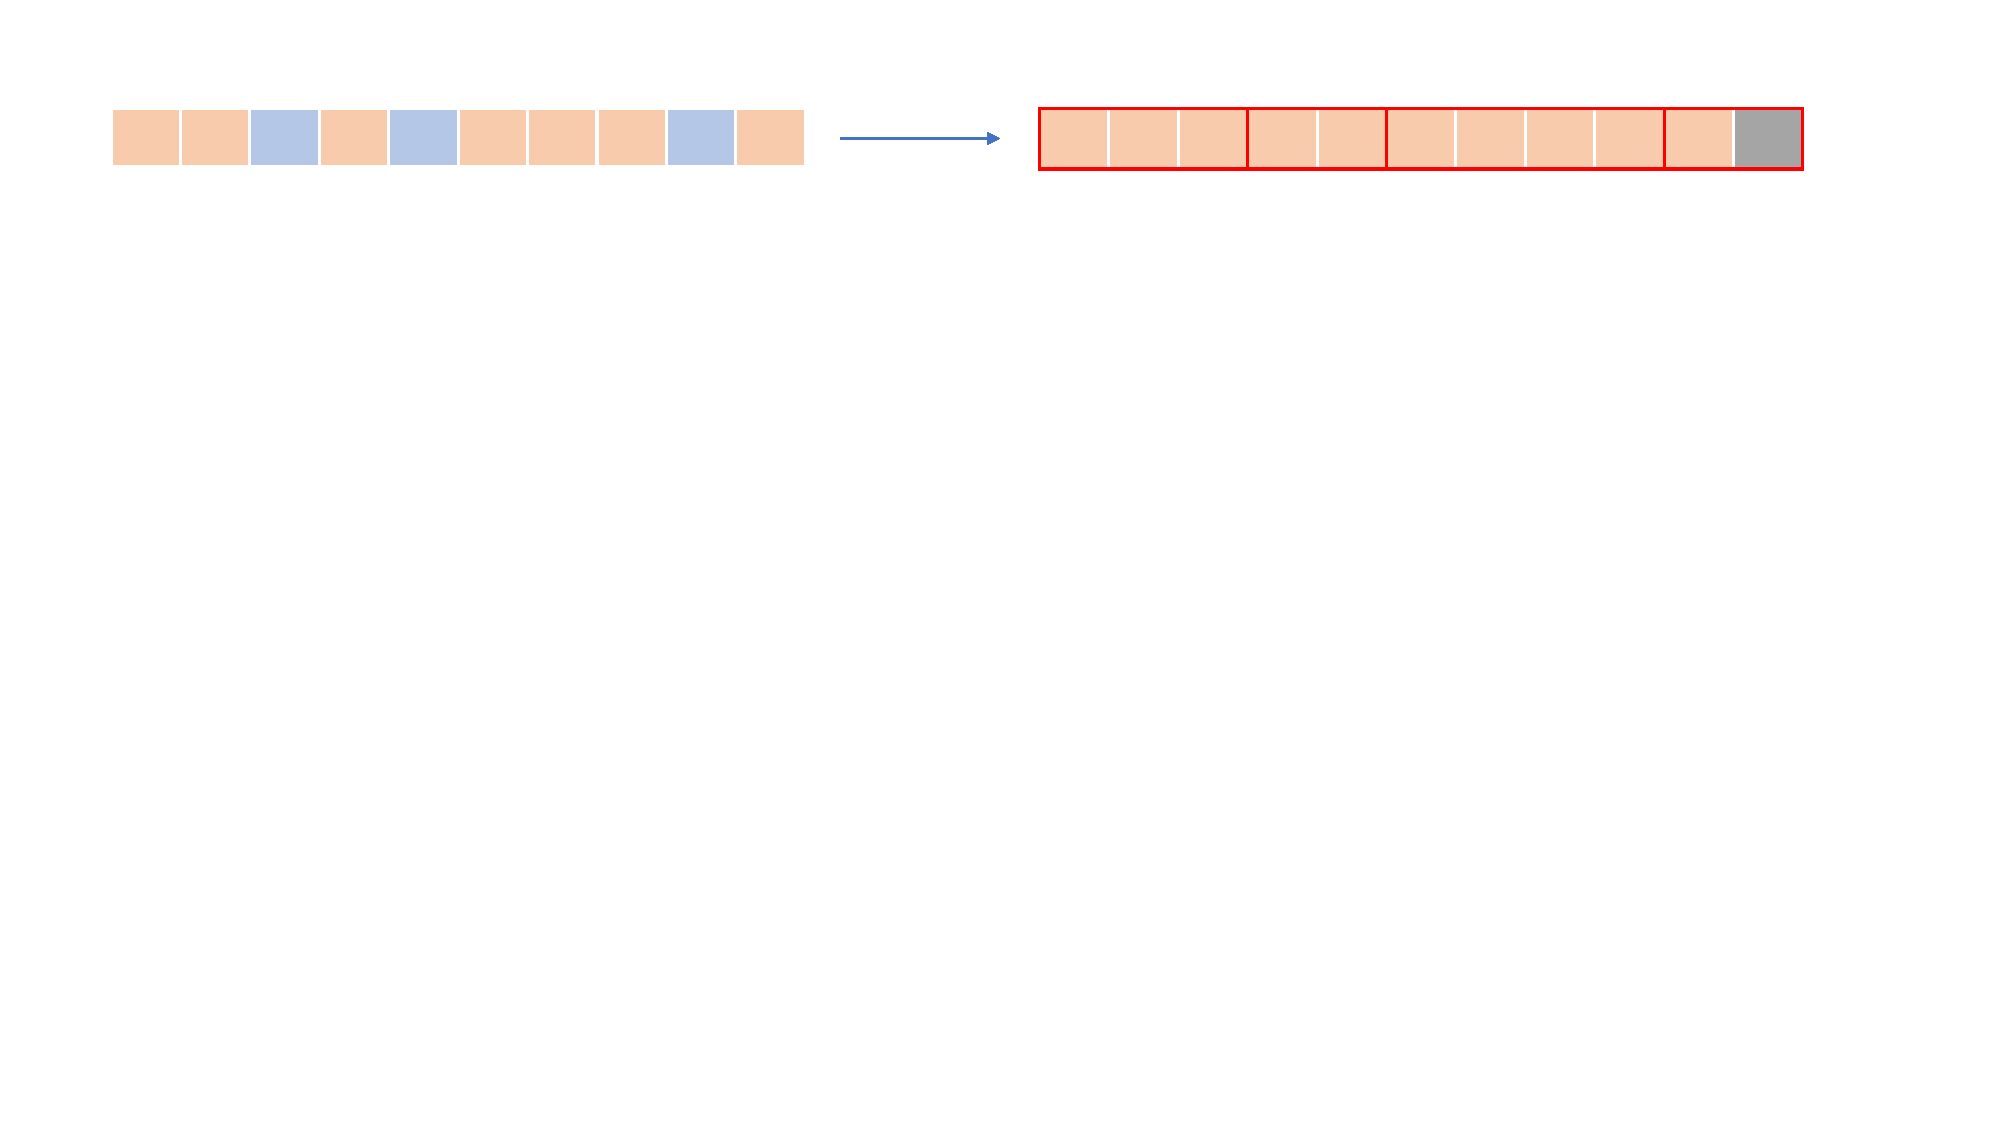
\includegraphics[width=0.8\textwidth]{./Figures/dummy_seat.pdf}
    \caption{Problem Conversion with One Seat as Social Distancing}
\end{figure}

After the conversion, $L = L^{0} + 1 =11$, $n_i = i + 1$ for $i = 1, 2, 3, 4$. For the first group, we use a group of three seats to indicate the original group of two and one seat used as the social distancing. We do the same procedure for the other groups. Then, the row can be represented by $\bm{h} = (2,1,1,0)$. The number of people that can be accommodated is $|\bm{h}| = 7$.

\end{example}


% We also introduce the concept of loss, which is the number of unoccupied seats. Mathematically, the loss is defined as $L- \delta - |\bm{h}|$, where $L$ denotes the length of the row.

\begin{definition}
Given the length of a row, denoted as $L$, and the maximum size of a group allowed, denoted as $M$, we can define certain characteristics of a pattern $\bm{h} = (h_1, \ldots, h_M)$.
We refer to a pattern $\bm{h}$ as a full pattern if it satisfies the condition $\sum_{i=1}^{M} n_i h_i = L$. Furthermore, we define a pattern $\bm{h}$ as a largest pattern if it has a size $|\bm{h}|$ that is greater than or equal to the size $|\bm{h}^{\prime}|$ of any other feasible pattern $\bm{h}^{\prime}$.
\end{definition}

In other words, a full pattern is one in which the sum of the product of the number of occurrences $h_i$ and the size $n_i$ of each group in the pattern is equal to the length of the row $L$. This ensures that the pattern fully occupies the available row seats. A largest pattern is one that either has the maximum size or is equal in size to other patterns, ensuring that it can accommodate the most number of people within the given row length.


\begin{prop}\label{lem_pattern}
Given the parameters of a row, including its length $L$, the social distancing requirement $\delta$, and the maximum size of a group allowed $M$, for one possible largest pattern $\bm{h}$, the maximum number of people that can be accommodated is given by $|\bm{h}| = qM + \max\{r-\delta, 0\}$, where $q = \lfloor \frac{L}{M + \delta} \rfloor$, $r \equiv L \bmod (M + \delta)$. 
\end{prop}

% The corresponding loss of the largest pattern equals $q \delta - \delta + \min\{r, \delta\}$, represents the amount of empty seats due to the social distancing requirement. 

The largest pattern $\bm{h}$ is unique and full when $r = 0$, indicating that only one pattern can accommodate the maximal number of people. On the other hand, if $r > \delta$, the largest pattern $\bm{h}$ is full, as it utilizes the available space up to the social distancing requirement.


\begin{example}
Consider the given values: $\delta = 1$, $L = 21$, and $M = 4$. In this case, we have $n_i = i + 1$ for $i = 1, 2, 3, 4$. The size of the largest pattern can be calculated as $qM + \max\{r-\delta, 0\} = 4 \times 4 + 0 = 16$. The largest patterns are the following: $(1, 0, 1, 3)$, $(0, 1, 2, 2)$, $(0, 0, 0, 4)$, $(0, 0, 4, 1)$, and $(0, 2, 0, 3)$.

The following figure shows that the largest pattern may not be full and the full pattern may not be largest.
\begin{figure}[ht]
    \centering
        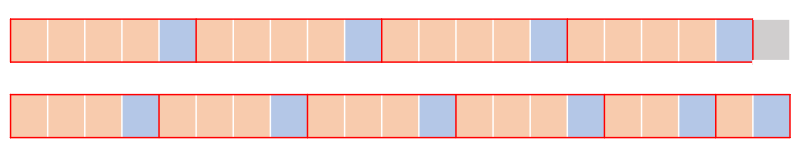
\includegraphics[width=0.8\textwidth]{./Figures/full_largest.png}
    \caption{Full and Largest Pattern}
\end{figure}

The first row can be represented by $(0, 0, 0, 4)$. It is a largest pattern as it can accommodate the maximum number of individuals. However, it does not satisfy the requirement of fully utilizing all available seats since $4 \times 5 \neq 21$.
The second row can be represented by $(1, 1, 4, 0)$, which is a full pattern as it utilizes all available seats. However, its size is 15, indicating that it is not the largest pattern.
\end{example}

% Through the above example, we observe that the largest pattern does not exclusively consist of large groups but can also include smaller groups. This highlights the importance of considering the various group sizes when using the largest pattern. Another observation relates to the relationship between the largest patterns and full patterns. It is apparent that a full pattern may not necessarily be the largest pattern. 

\newpage